\section{Versuchsaufbau}
\label{sec:Versuchaufbau}
In diesem Kapitel werden alle in diesem Versuch verwendeten elektronischen Schaltungen für die Modulation als auch die Demodulation beschrieben und erläutert.
\subsection{Modulation}
\subsubsection{Primitive Modulatorschaltung mittels Diode}
Zur Realisierung einer Amplitudenmodulation wird eine Schaltung benötigt, die die Trägerspannung mit der Modulationsspannung multipliziert. Eine solcher Aufbau ist in Abbildung XXX dargestellt.

% \begin{figure}
%     \centering
%     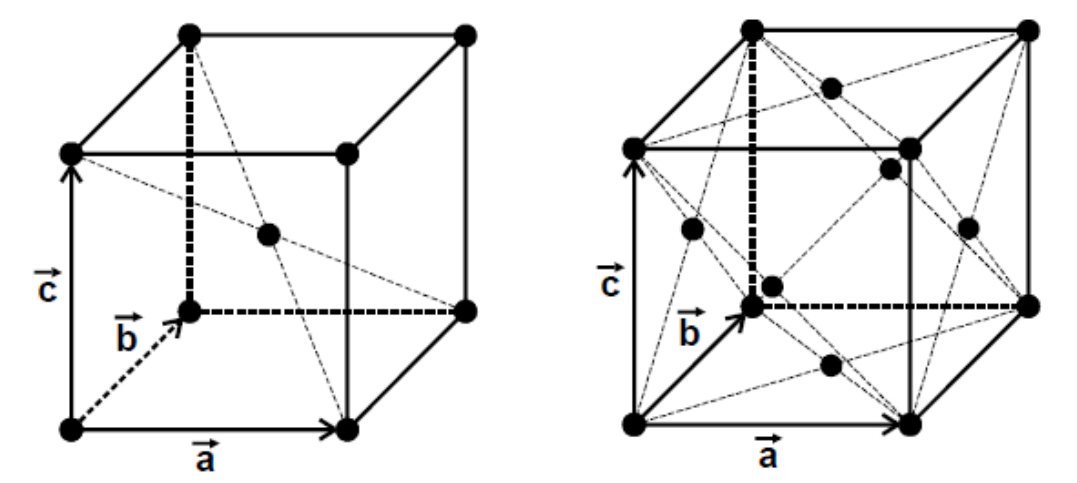
\includegraphics[width=0.55\textwidth]{ressources/kubies.png}
%     \caption{Abbildung eines bcc-Gitters (links) und eines fcc-Gitters\cite{skript}.}
%     \label{bcc}
% \end{figure}

Durch die nicht lineare Diodenkennlinie entstehen während der Multiplikation durch die Potenzreihenentwicklung unerwünschte Therme höherer Ordnung der Träger- und Modulationsspannung. Dessen Frequenzen liegen außerhalb des Intervalls $[\omega_T-\omega_M, \omega_T+\omega_M]$ und können somit durch Bandfilter unterdrückt werden.

\subsubsection{Ringmodulator}
Durch den sogenannten Ringmodulator, siehe Abbildung XXX, sind die bei der Schaltung im vorherigen Kapitel unerwünscht enstandenen Komponenten zu vermeiden. Wie in Abbildung XXX dargestellt, sind die vier Dioden der Hauptbestandteil der Schaltung. 

% \begin{figure}
%     \centering
%     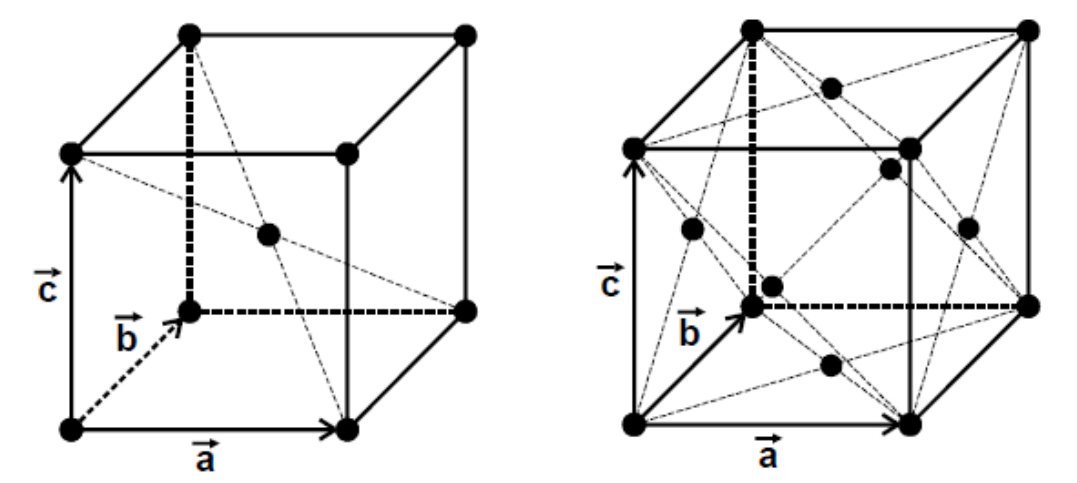
\includegraphics[width=0.55\textwidth]{ressources/kubies.png}
%     \caption{Abbildung eines bcc-Gitters (links) und eines fcc-Gitters\cite{skript}.}
%     \label{bcc}
% \end{figure}

Durch diese wird eine Spannungsteiler an den Punkten $\alpha$ und $\beta$ realisiert, wodurch, bei baugleichen Dioden und ohne anliegender Modulationsspannung, keine Potentialdifferenz zwischen dem beiden besagten Punkten auftritt. Erst durch das anlegen einer Modulationsspannung $U_M$ wird das Gleichgewicht gestört und die Teilungsverhältnisse der Dioden schwinken im Rhythmus von $U_M(t)$. Bei idealen Verhältnissen ist somit das Produkt der Eingangsspannungen proportional zur Ausgangsspannung. Zusätzlich entsteht bei dem Ringmodulator keine Trägerabstrahlung, weshalb nur die Seitenbänder entstehen.

\subsubsection{Frequenzmodulator mit geringem Frequenzhub}
Grundlage ist hierfür der in Kapitel XXX beschriebene Ringmodulator. Da durch diesen nur die Seitenbändern ohne Trägerabstrahlung erzeugt wird, muss die Trägerfrequenz mit einer Phasenverschiebung von $\pi/2$ gesondert hinzugefügt werden. Dieses wird, wie in Abbildung XXX dargestellt, über ein Laufzeitkabel von $\SI{250}{\ns}$ realisiert. 

% \begin{figure}
%     \centering
%     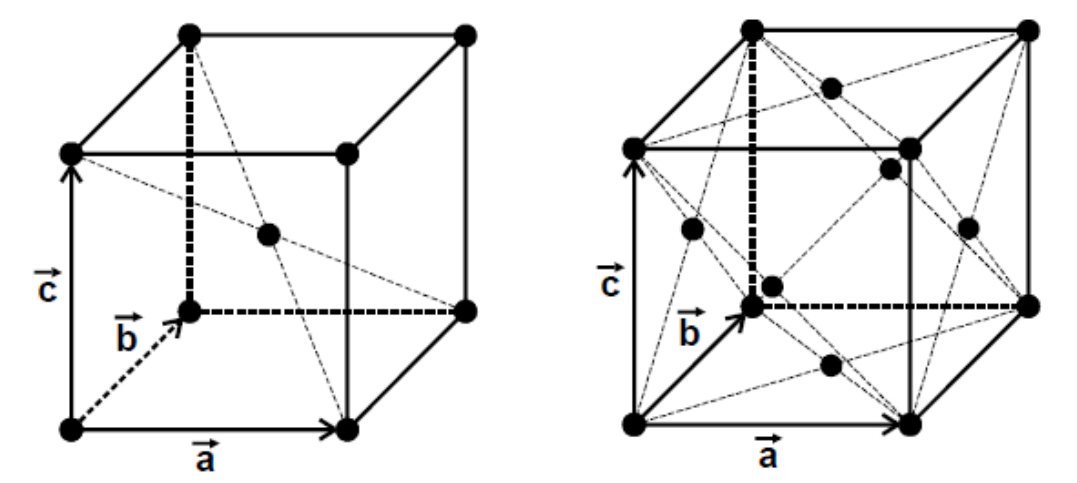
\includegraphics[width=0.55\textwidth]{ressources/kubies.png}
%     \caption{Abbildung eines bcc-Gitters (links) und eines fcc-Gitters\cite{skript}.}
%     \label{bcc}
% \end{figure}

Um die gewünschte Phasenverschiebung zu erhalten, kann über die gegebene Periodendauer die benötigte Frequenz bestimmt werden.

\subsection{Demodulation}

\subsection{Demodulation amplitudenmodulieter Schwingungen}
Zur Demodulation wird ebenfalls ein Ringmodulator verwendet. Wie in Abbildung XXX dargestellt, ist am Eingang L die modulierte Spannung und am Eingang R die Trägerspannung angelegt. 

% \begin{figure}
%     \centering
%     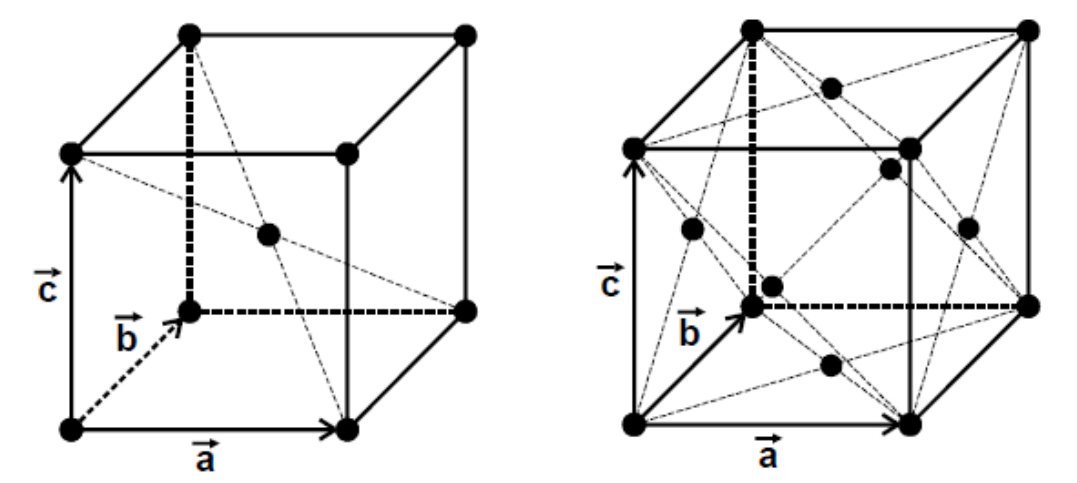
\includegraphics[width=0.55\textwidth]{ressources/kubies.png}
%     \caption{Abbildung eines bcc-Gitters (links) und eines fcc-Gitters\cite{skript}.}
%     \label{bcc}
% \end{figure}

Da die Frequenz der Eingänge addiert und subtrahiert werden ergeben sich aus den angelegten Frequenzen $\omega_T\pm\omega_M$ (Eingang L) und $\omega_T$ (Eingang R) am Ausgang X die Frequenzen $2\omega_T\pm\omega_M$ und $\omega_M$.

\subsection{Demodulator-Schaltung mit einer Gleichrichter-Diode}
Ein weiteres Verfahren zur Demodulation einer Amplitudenmodulation besteht in der Verwendung einer Gleichrichterdiode mit geeignetem Tiefpass. Diese Schaltung findet Anwendung wenn die ursprüngliche Trägerspannung nicht zur Demodulation zur Verfügung steht. Wie in Abbildung XXX dargestellt, werden durch die Diode sämtliche negativen Halbwellen der Signalspannung entfernt.

% \begin{figure}
%     \centering
%     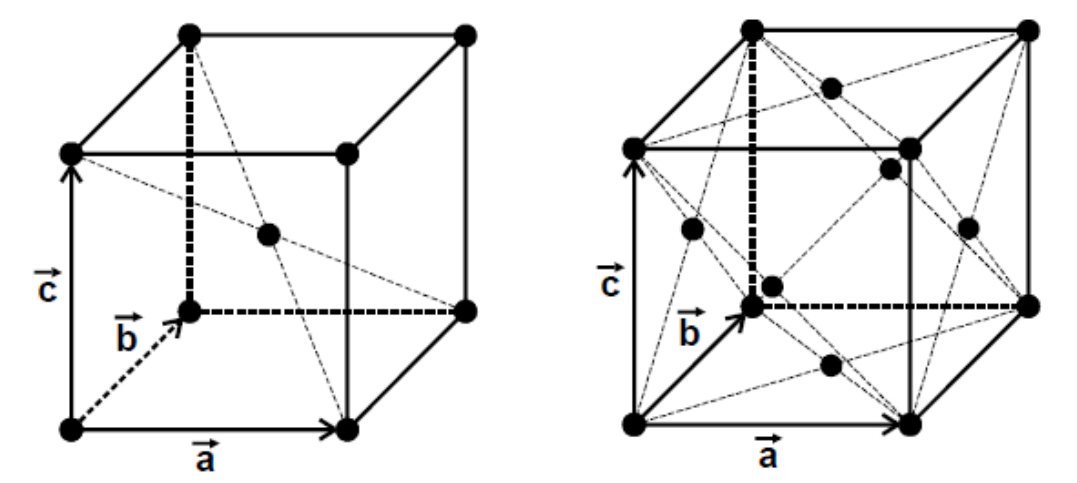
\includegraphics[width=0.55\textwidth]{ressources/kubies.png}
%     \caption{Abbildung eines bcc-Gitters (links) und eines fcc-Gitters\cite{skript}.}
%     \label{bcc}
% \end{figure}

Die in Abbildung XXX dargestellte Spannung am Punkt A enthält zu diesem Zeitpunkt hochfrequente Anteile der Form $\omega_T$, $2\omega_T$, $4\omega_T$ u.s.w. und $\omega_M$. Da die Beziehung $\omega_T>>\omega_M$ weiterhin gilt, kann die hohe Trägerfrequenz und deren vielfache durch einen Tiefpass unterdrückt werden, sodass die in Abbildung XXX dargestellte Modulationsfrequenz extrahiert werden kann. 

% \begin{figure}
%     \centering
%     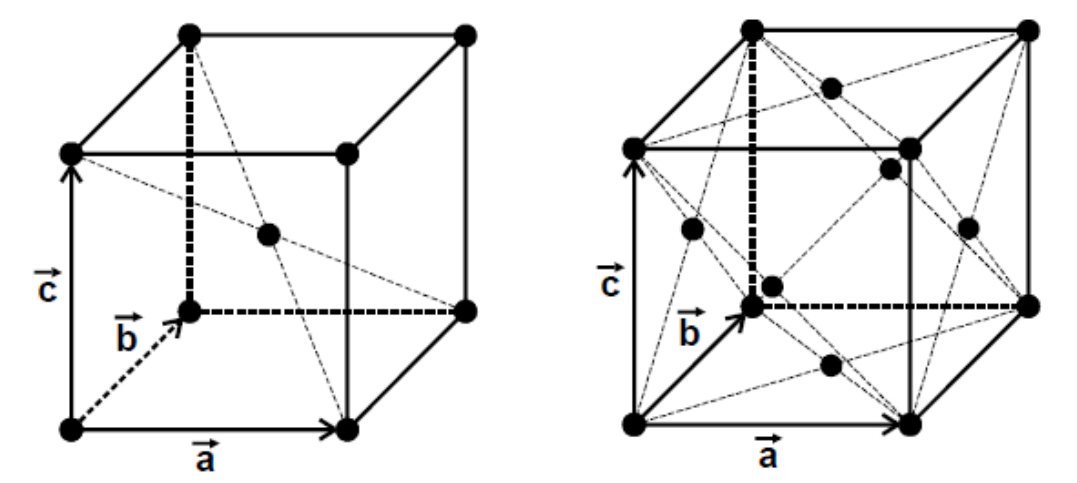
\includegraphics[width=0.55\textwidth]{ressources/kubies.png}
%     \caption{Abbildung eines bcc-Gitters (links) und eines fcc-Gitters\cite{skript}.}
%     \label{bcc}
% \end{figure}

% \begin{figure}
%     \centering
%     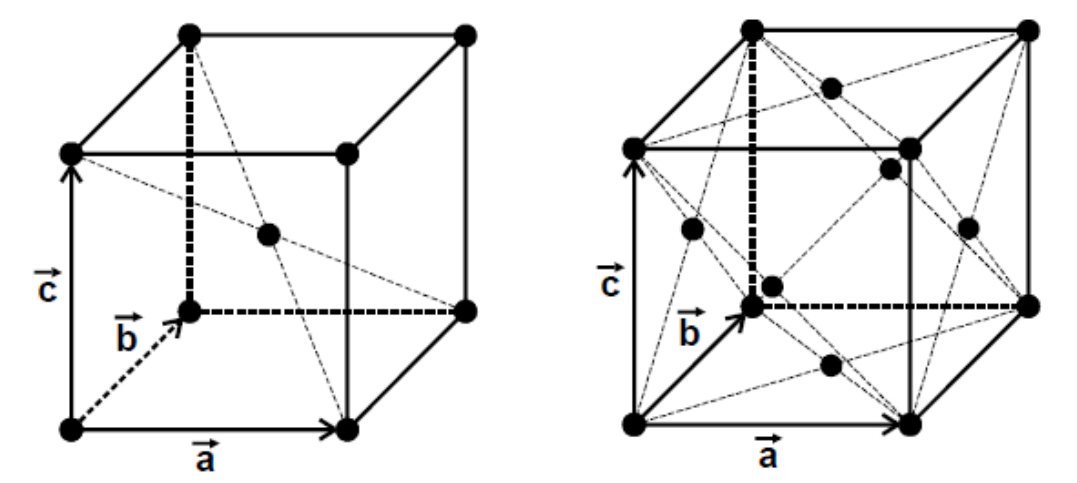
\includegraphics[width=0.55\textwidth]{ressources/kubies.png}
%     \caption{Abbildung eines bcc-Gitters (links) und eines fcc-Gitters\cite{skript}.}
%     \label{bcc}
% \end{figure}

In der Realität ist die erhaltene Frequenz jedoch verzerrt gegenüber der ursprünglichen Modulationsfrequenz, da die Diode eine annähernd exponentiellen Kennlinienverlauf aufweißt. Wird jedoch eine sehr kleine Modulationsfrequenz gewählt, kann die Kennlinie der Diode linear genähert werden und so eine Verzerrung vermindert werden.

\subsection{Demodulation frequenzmodulieter Schwingungen}
Im ersten Teil der Demodulation findet die Umwandlung  in eine amplitudenmodulierte Schwingung statt. Dieses wird durch einen LC-Schwingkreis realisiert, wie in Abbildung XXX zu sehen. 

% \begin{figure}
%     \centering
%     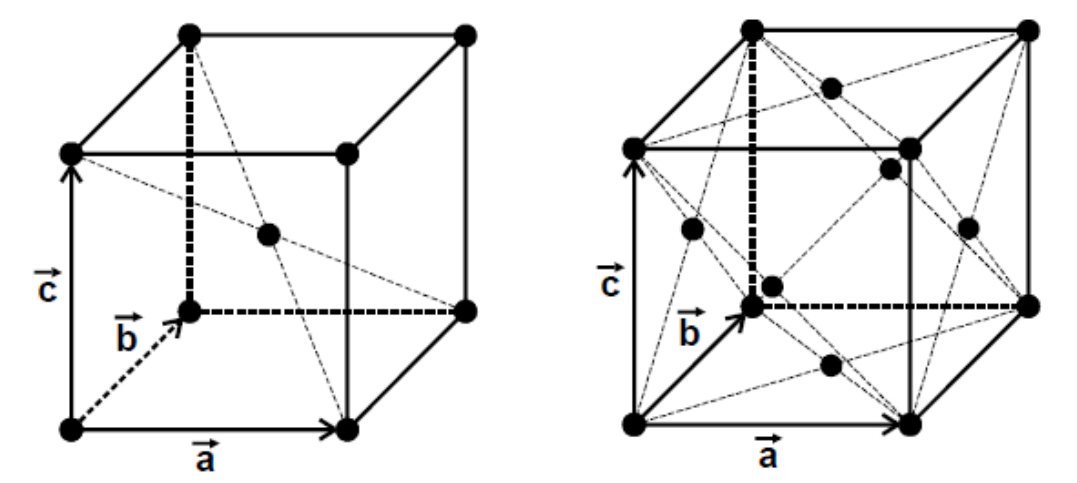
\includegraphics[width=0.55\textwidth]{ressources/kubies.png}
%     \caption{Abbildung eines bcc-Gitters (links) und eines fcc-Gitters\cite{skript}.}
%     \label{bcc}
% \end{figure}


Aus diesem Grund ist die Resonanzfrequenz der Schaltung so gewählt, dass Trägerfrequenz auf der Flanke der Resonanzkurve liegt (siehe Abbildung XXX). Ändert sich Momentanfrequenz der Schwingung, so ensteht am Ausgang der Schaltung eine hochfrequente Spannung, die keine konstante Amplitude mehr aufweißt sondern deren Amplitude im Rhytmus der Modulationsfrequenz schwinkt. Im zweiten Schritt ist die Demodulations der amplitudenmodulierten Schwingung durch in Kapitel XXX oder XXX vorgestellte Methoden durchzuführen. 

% \begin{figure}
%     \centering
%     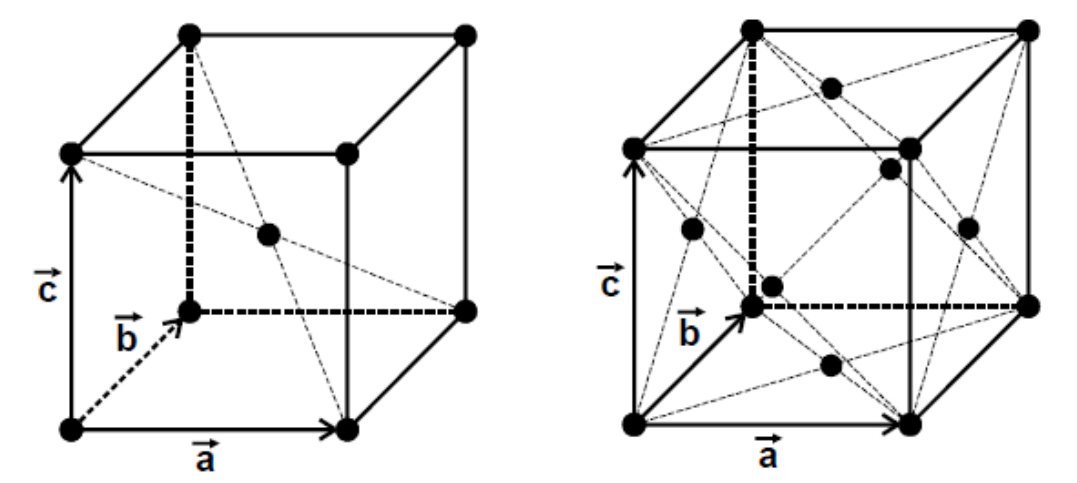
\includegraphics[width=0.55\textwidth]{ressources/kubies.png}
%     \caption{Abbildung eines bcc-Gitters (links) und eines fcc-Gitters\cite{skript}.}
%     \label{bcc}
% \end{figure}
